\documentclass[a4paper,12pt]{article}
\usepackage{url}
\usepackage{listings}
\usepackage{color}
\usepackage{hyperref}
\usepackage{graphicx}
\usepackage{booktabs}
%\usepackage{mdframed}
\usepackage{adjustbox}

\definecolor{dkgreen}{rgb}{0,0.6,0}
\definecolor{gray}{rgb}{0.5,0.5,0.5}
\definecolor{mauve}{rgb}{0.58,0,0.82}

\lstset{frame=tb,
	language=C++,
	aboveskip=3mm,
	belowskip=3mm,
	showstringspaces=false,
	columns=flexible,
	basicstyle={\small\ttfamily},
	numbers=none,
	numberstyle=\tiny\color{gray},
	keywordstyle=\color{blue},
	commentstyle=\color{dkgreen},
	stringstyle=\color{mauve},
	breaklines=true,
	breakatwhitespace=true,
	tabsize=3
}
\begin{document}

\title{CS-224 Object Oriented Programming and Design Methodologies }
\author{Assignment 04}
\date{Fall 2021}
\maketitle
\section{Guidelines}
You need to submit this assignment on  {\color{red}Nov 7 at 2359}. Some important guidelines about the assignment are as following:

\begin{itemize}
	\item You can do this assignment in a group of two students, and if you want you can also do it alone.
	\item You will submit your assignment to LMS (only one member of the group will submit).
	\item Clearly mention the group composition in submitted file name e.g. AhmadHassan\_ah01345\_BatoolAiman\_ba03451.zip.
	\item You need to follow the best programming practices
	\item Submit assignment on time; late submissions will not be accepted.
	\item Some assignments will require you to submit multiple files. Always Zip and send them.
	\item It is better to submit incomplete assignment than none at all.
	\item It is better to submit the work that you have done yourself than what you have plagiarized.
	\item It is strongly advised that you start working on the assignment the day you get it. Assignments WILL take time.
	      %		\item Every assignment you submit should be a single zipped file containing all the other files. Suppose your name is John Doe and your id is 0022 so the name of the submitted file should be JohnDoe0022.zip
	\item DO NOT send your assignment to your instructor, if you do, your assignment will get ZERO for not following clear instructions.
	\item You can be called in for Viva for any assignment that you submit
\end{itemize}




\section{BattleField}

A sample code is given in BattleField folder, if you run it you can see a bullet is created everytime you click on the screen, it is moving slightly towards right side. This example creates and display an object using SDL library. It uses \texttt{Bullet} class to create and draw an object. This class is inherited from \texttt{Unit} class that is fully implemented and takes care of all the drawing aspects, hence you don't need to change anything in it.

You are required to:
\begin{itemize}
	\item Create a class \texttt{TankTurret}, this class will be displaying a tank turret, and can be implemented similar to \texttt{Bullet}.
	\item Create a class \texttt{TankBody}, this class will be displaying a tank body, and can be implemented similar to \texttt{Bullet}.
	\item Create a class \texttt{Tank}, this class makes a composition of TankTurret and TankBody objects, i.e. in each Tank there is a tankBody and a tankTurret object.
	\item When you click on the screen, a Tank object is created dynamically instead of a Bullet. Remember that the tank object should be created by using new operator, hence the list of tanks will also be storing pointers of tanks.
	\item When you press \texttt{F key}, it fires bullets from all the tanks displayed on the screen. It means, at pressing the F key, you have to create one bullet object corresponding to each Tank being currently displayed. The bullets will also be created dynamically, and would be stored in a list. Here the list type would be pointers to Bullet.
	\item Tank should make an animation to move its turret slightly towards left, when a bullet is fired, then it returns back to its position.
	\item Modify the Bullet class, so that it displays a vanishing animation when it reaches to right most corner of the screen. Look at the different bullet animations in the assets file.
	      
	\item Remember to remove the objects from memory when they are not in use any more.
\end{itemize}


\begin{figure}
	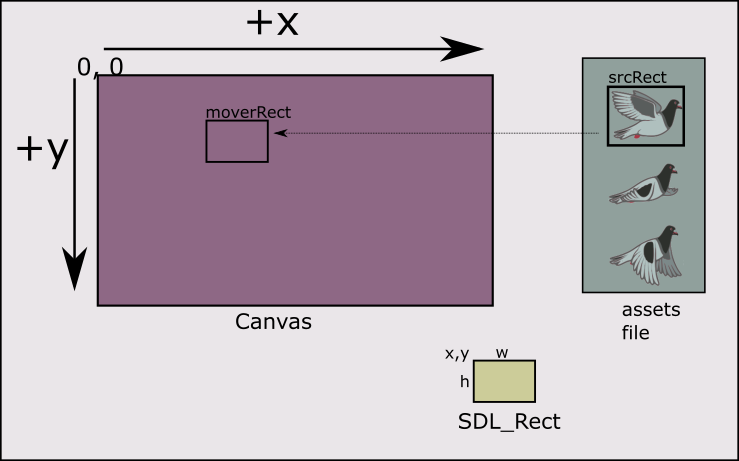
\includegraphics[width=\linewidth]{sdlDrawing}
	\caption{SDL Drawing Basics}
	\label{fig:sdlDrawing}
\end{figure}



\subsection{SDL Drawing Basics}

The basic drawing function in SDL is very simple, you need two SDL\_Rect variables to draw a portion of image from assets file to the canvas. \texttt{SDL\_Rect} is a simple structure containing \texttt{\{x, y, w, h\} }attributes. \texttt{(x, y)} is the top-left corner, and \texttt{w, h} are width and height of rectangle. You define a \texttt{srcRect} for desired object in assets file, and define a \texttt{moverRect} for this image to be drawn on desired location on canvas. Refer to Figure \ref{fig:sdlDrawing} for all this process.  Finally you call 

\noindent \texttt{SDL\_RenderCopy(gRenderer, assets, \&pigeonSrc, \&pigeonMover);}

\noindent that displays this image to the canvas, voila!!!. Refer to \texttt{assets.png} file for all the required image assets.

You can draw as many objects in the \texttt{HUMania.cpp $ \Rightarrow $ drawObjects()}, as you want. Since this function is called infinitely, you can change the \texttt{x, y} attributes of \texttt{moverRect} to move the objects on screen, and you can change the \texttt{srcRect} values to get a flying animation.



\section{\texttt{std::list} Tutorial}

Following is a basic example to work with vector. Complete reference for C++ vector is given here \url{https://en.cppreference.com/w/cpp/container/vector}
\begin{lstlisting}
#include<iostream>
#include<list>

using namespace std;

class Distance{
	int feet, inches;
	public:
	Distance(int ft, int inch): feet(ft), inches(inch){}
	void show(){
		cout<<feet<<"'"<<inches<<"\""<<endl;
	}
};

int main(){
	list<Distance*> dst; // It's a vector that can store Distance type objects
	dst.push_back(new Distance(3, 4)); // create an object, and push it in vector
	dst.push_back(new Distance(5, 2));
	dst.push_back(new Distance(2, 7));
	dst.push_back(new Distance(7, 8));
	dst.push_back(new Distance(13, 1));
	
	for(int i=0;i<dst.size();i++)
		dst[i]->show(); // call show method of dst[i] object
		
	for(int i=0;i<dst.size();i++)
		delete dst[i]; // Let's delete all the objects
		
	// all the objects are deleted, but dst still holds the pointers	
	dst.clear(); // It clears up all the pointers stored in dst
}

//////////////// Output: ///////////////////
3'4"
5'2"
2'7"
7'8"
13'1"
	\end{lstlisting}

\section{Some important points:}

\begin{itemize}
	\item Sample code is there for your benefit. If you are going to use it, understand how it works.
	\item You do not need to follow the code given exactly. You can make changes where you see fit provided that it makes sense.
	\item Make the class declarations in hpp files, and provide function implementations in cpp files. Don't use hpp files for implementation purposes.
	      %		\item Implement Q1 prior to implementing Q2, it will help you to implement linked list.
	      %		\item Where necessary, declare your own functions inside classes. Make sure why you would keep a function as private or public.
	\item As a general rule, class's deta is private, and functions are public. Don't use getter/setter functions to manipulate data, rather think in object oriented directions and provide all the functionality in the class.
	\item Complete reference for C++ vector is given here \url{https://en.cppreference.com/w/cpp/container/vector}
	\item You need to define separate \path{*.hpp} and \path{*.cpp} files for all the classes.
	\item Exact x,y,w,h values for images in assets file can be found by \url{http://www.spritecow.com/}.
	\item A tutorial for file I/O is given \url{http://www.cplusplus.com/doc/tutorial/files/}.
	\item You should take \url{www.cplusplus.com} and \url{www.cppreference.com} as primary web source to search about C++
	\item You have to follow best OOP practices as discussed in lectures.
\end{itemize}



\section{Rubric}
\begin{table}[!h]
	\centering
	\begin{tabular}{llc}
		\toprule
		%Warnings/Errors	& The code had no warnings/errors	& 1 \\
		Comments      & The code was properly commented                         & 1  \\
		Coding        & The code followed best practices guideline              & 2  \\
		OOP Concepts  & The code followed best OOP practices                    & 3  \\
		% Modularization &	Code is modularized in different functions	& 1\\
		Functionality & All the functionality is implemented as described above & 4  \\
		\midrule
		Total         &                                                         & 10 \\
		\bottomrule
	\end{tabular}
	\caption{Grading Rubric}
	\label{Grading}
\end{table}


\newpage


\end{document}